\subsection{Learning Theories in Simulation-Based XR}


\subsubsection{Experiential Learning in an XR environment}

Experiential learning theory posits that learning is a process through which knowledge is created via the transformation of experience \parencite{kolb1984}. This perspective emphasizes that learning emerges through the integration of experiencing, reflecting, thinking, and acting within a continuous cycle.

Kolb conceptualizes learning as a four-stage cyclical process consisting of concrete experience (CE), reflective observation (RO), abstract conceptualization (AC), and active experimentation (AE) \parencite{almeida_learning_2010}, as illustrated in \cref{fig:exp4stages}.

Concrete experience refers to the learner's direct engagement in a specific activity, where immersive technologies such as extended reality (XR) can enhance the sense of presence. Reflective observation involves consciously reflecting on the experience, often supported by feedback mechanisms or guidance;in this context, a human-AI collaboration agent can provide timely and accurate support to help learners interpret their experiences. Abstract conceptualization entails the formation or refinement of theoretical constructs and hypotheses derived from reflection. Finally, active experimentation involves applying these conceptualizations to new situations, allowing learners to test their understanding and generate new experiences, thereby continuing the learning cycle.


\begin{figure}[H]
\caption{The Four-Stage Learning Cycle by Kolb (1984)}\label{fig:exp4stages}
\centering
\centering
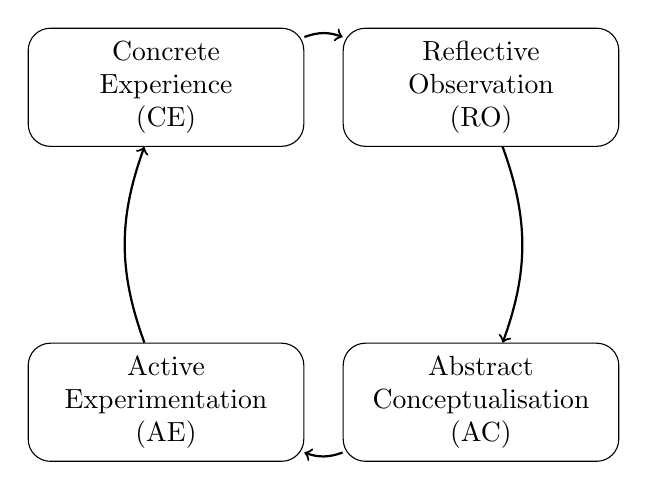
\begin{tikzpicture}[
    node distance=4cm,
    every node/.style={
        draw,
        rounded corners=8pt,
        minimum width=3.5cm,
        minimum height=1.5cm,
        align=center
    },
    arrow/.style={->, thick}
]

% Nodes
\node (ce) {Concrete\\Experience\\(CE)};
\node (ro) [right of=ce] {Reflective\\Observation\\(RO)};
\node (ac) [below of=ro] {Abstract\\Conceptualisation\\(AC)};
\node (ae) [left of=ac] {Active\\Experimentation\\(AE)};

% Arrows
\draw[arrow] (ce) to[bend left=20] (ro);
\draw[arrow] (ro) to[bend left=20] (ac);
\draw[arrow] (ac) to[bend left=20] (ae);
\draw[arrow] (ae) to[bend left=20] (ce);

\end{tikzpicture}
\end{figure}


Prior research suggests that virtual reality (VR), as an experiential learning tool, can effectively enhance technical skills and learner confidence, even with relatively short exposure times \parencite{knobovitch_virtual_2025}. VR also enables personalized learning experiences by allowing students to explore virtual environments at their own pace and according to their individual preferences. Furthermore, VR systems can support improved comprehension through the delivery of adaptive and personalized feedback \parencite{marougkas_virtual_2023}.

In addition, the immersive and interactive nature of XR has been shown to promote higher levels of engagement, both physically and cognitively \parencite{liu_research_2025}. Compared with flat display devices, XR-based approaches can also improve learner concentration. For example, \textcite{liu_research_2025} found that learners in a VR-based instruction (VRI) group demonstrated higher task mastery rates than those in other groups. This improvement was attributed to increased engagement and interactivity, which supported better information retention.

\subsubsection{FPV Training Simulators}

Training Simulators are designed to imitate the operations and behaviors of a facility or process, so as to develop the skills or experiences of the operators who use them. The objective of the operator of the Training Simulator is to maximize his performance in achieving the task being simulated.\parencite{narayanasamy_distinguishing_2006}. Simulation-based learning as an active and immersive experience in a virtual learning environment that recreate a realistic and authentic real-life event or a set of learning situations to solve a problem.\parencite{dai_educational_2022}

In aviation and drone domains, such systems replicate flight dynamics, cockpit instrumentation, and environmental conditions of real aircraft. Flight training simulators have a long history, beginning around 1910 and evolving significantly during the World Wars. By the 1960s, they had become essential tools for pilot training, enabling the safe practice of complex scenarios. With advances in artificial intelligence and related technologies, modern simulators can now provide real-time feedback based on expert pilot performance. Today, they are widely used in both civilian and military contexts for training and mission planning \parencite{pappas_generic_2025}.

An FPV (First-Person View) training simulator is a specialized computer-based training system designed to teach and refine the technical skills required to operate FPV drones. Similar to traditional flight simulators, FPV simulators are widely used across entertainment, professional training, and research contexts. 

Existing literature on drone simulators has primarily focused on technical design or training effectiveness, often using research-oriented platforms such as Microsoft AirSim. However, widely used commercial FPV simulators (e.g., Liftoff and Uncrashed) remain under explored in pedagogical research. These commercial simulators typically emphasize high-fidelity environments and support advanced flight modes such as acrobatic mode for pilot practice. In contrast, research platforms such as AirSim and RotorS are widely used for machine learning and autonomous system development, but are not specifically tailored for practical pilot training \parencite{pappas_generic_2025}.

Despite their realism, FPV simulators also present several limitations. For example, while they aim to replicate real-world physics, users often report a steep learning curve and highly unforgiving flight dynamics, which may not always support beginner training effectively \parencite{guide_best_2026}. Additionally, hardware compatibility issues can arise, as not all radio transmitters are universally supported. The lack of standardization in flight controller architectures, along with the prevalence of proprietary and closed-source systems in UAV platforms, further complicates integration and usability \parencite{ebeid_survey_2018}.


\subsubsection{Learning in Extended Reality (XR)}

\parencite{emma_extended_2026}
\parencite{lowell_extended_2024}
\parencite{curran_use_2022}
\parencite{curran_use_2024}
\parencite{chen_effects_2022}
\parencite{zwolinski2022xr}

%------Need Checking--------------%
% Experiential Learning（Kolb）
% → XR enables “learning by doing”
% → XR creates:
% immersion
% safe training environment
% → apply：
% simulation-based learning
% skill acquisition（比如 drone control）

\subsubsection{Human-AI Collaboration}

\parencite{yin_ai_2023}
\parencite{gao2025humancenteredhumanaicollaborationhchac}
%------Need Checking--------------%

\subsubsection{Reinforcement Learning (RL)}

While Proportional-Integral-Derivative (PID) control is the industry standard for stable piloting. 
It offers a simple, white-box solution mentioned before. 
But it often struggles with complex situations where the Integral term alone is insufficient. 
Recently, Reinforcement Learning (RL) has gained traction as a robust black-box alternative. 
To reduce the computational burden on onboard systems, reinforcement learning has increasingly been adopted as a key approach for autonomous obstacle avoidance \parencite{yu2025depth}.

The concept of implementing RL in computing is among the earliest visions of AI.In a 1948 report, Alan Turing described a design for a pleasure-pain system \parencite{barto2019rl}. 
Modern RL defines a framework where an agent learns behavior through trial-and-error interactions with a dynamic environment \parencite{kaelbling1996rl}. 
Unlike supervised learning, the agent is not provided with correct answers.
Instead, it receives a scalar reinforcement signal (reward or punishment) and must discover actions that maximize its long-term cumulative reward.

Markov Decision Processes (MDPs) provide the mathematical foundation for RL.In an MDP, an agent's actions influence both the immediate reward and the subsequent state of the environment. An MDP shown in \cref{fig:MDP} is formally defined by (1) A set of states (S): Possible environment configurations; (2) A set of actions (A): Choices available to the agent;(3) A reward function (R): $R: S \times A \to \mathbb{R}$, specifying the instantaneous reward; (4) A state transition function (T): $T: S \times A \to \Delta(S)$, defining the probability of transitioning to state $s'$ given action $a$ in state $s$.

\begin{figure}
    \caption{Markov Decision Process diagram}
    \label{fig:MDP}
    \centering
    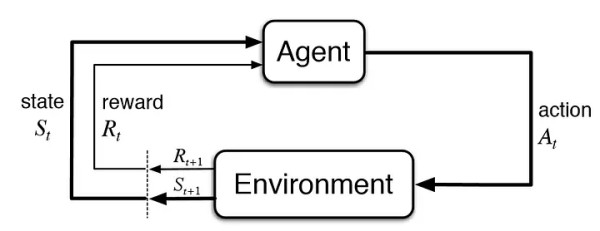
\includegraphics[width=0.8\linewidth]{img/decision.jpg}
\end{figure}

For training simulators, reinforcement learning can be used as a new way to build co-training agents.